% -*- LaTeX -*-
% -*- coding: utf-8 -*-
%
% michael a.g. aïvázis <michael.aivazis@para-sim.com>
% (c) 2003-2017 all rights reserved
%

\section{components}
\subsection{basics}

% --------------------------------------
% components:
\begin{frame}
%
  \frametitle{Extending object oriented ideas}
%
  \begin{itemize}
%
  \item most of the \pyre\ services are organized using \emph{objects}
%
  \item informally, \emph{classes} are software specifications that establish a relationship
    between \emph{state} and \emph{behavior}
    \begin{itemize}
    \item we have syntax that allows us to specify these very close to each other
    \end{itemize}
%
  \item \emph{instances} are containers of state; there are special rules
    \begin{itemize}
    \item that grant access to this state
    \item allow you to call functions that get easy access to this state
    \item it is worth remembering that python classes are themselves live objects: they
      are instances of their \emph{type}
    \end{itemize}
%
  \item these ideas have been around for a while\supercite{dahl-66,eiffel}, and have been
    explored extensively and formalized\supercite{meyer-97}
%
  \item \pyre\ \emph{components} are classes that specifically grant access to some of their
    state to the end user
    \begin{itemize}
    \item the public data are the \emph{properties} of the component
    \end{itemize}
%
  \item the notion is quite old\supercite{mcilroy-69} and the terms heavily overloaded; \pyre\
    components are an evolution of these ideas
%
  \end{itemize}
%
\end{frame}

\subsection{design}
%-----------------------------------
\begin{frame}
%
  \frametitle{SRTM -- the module}
%
  \begin{center}
    \only<1>{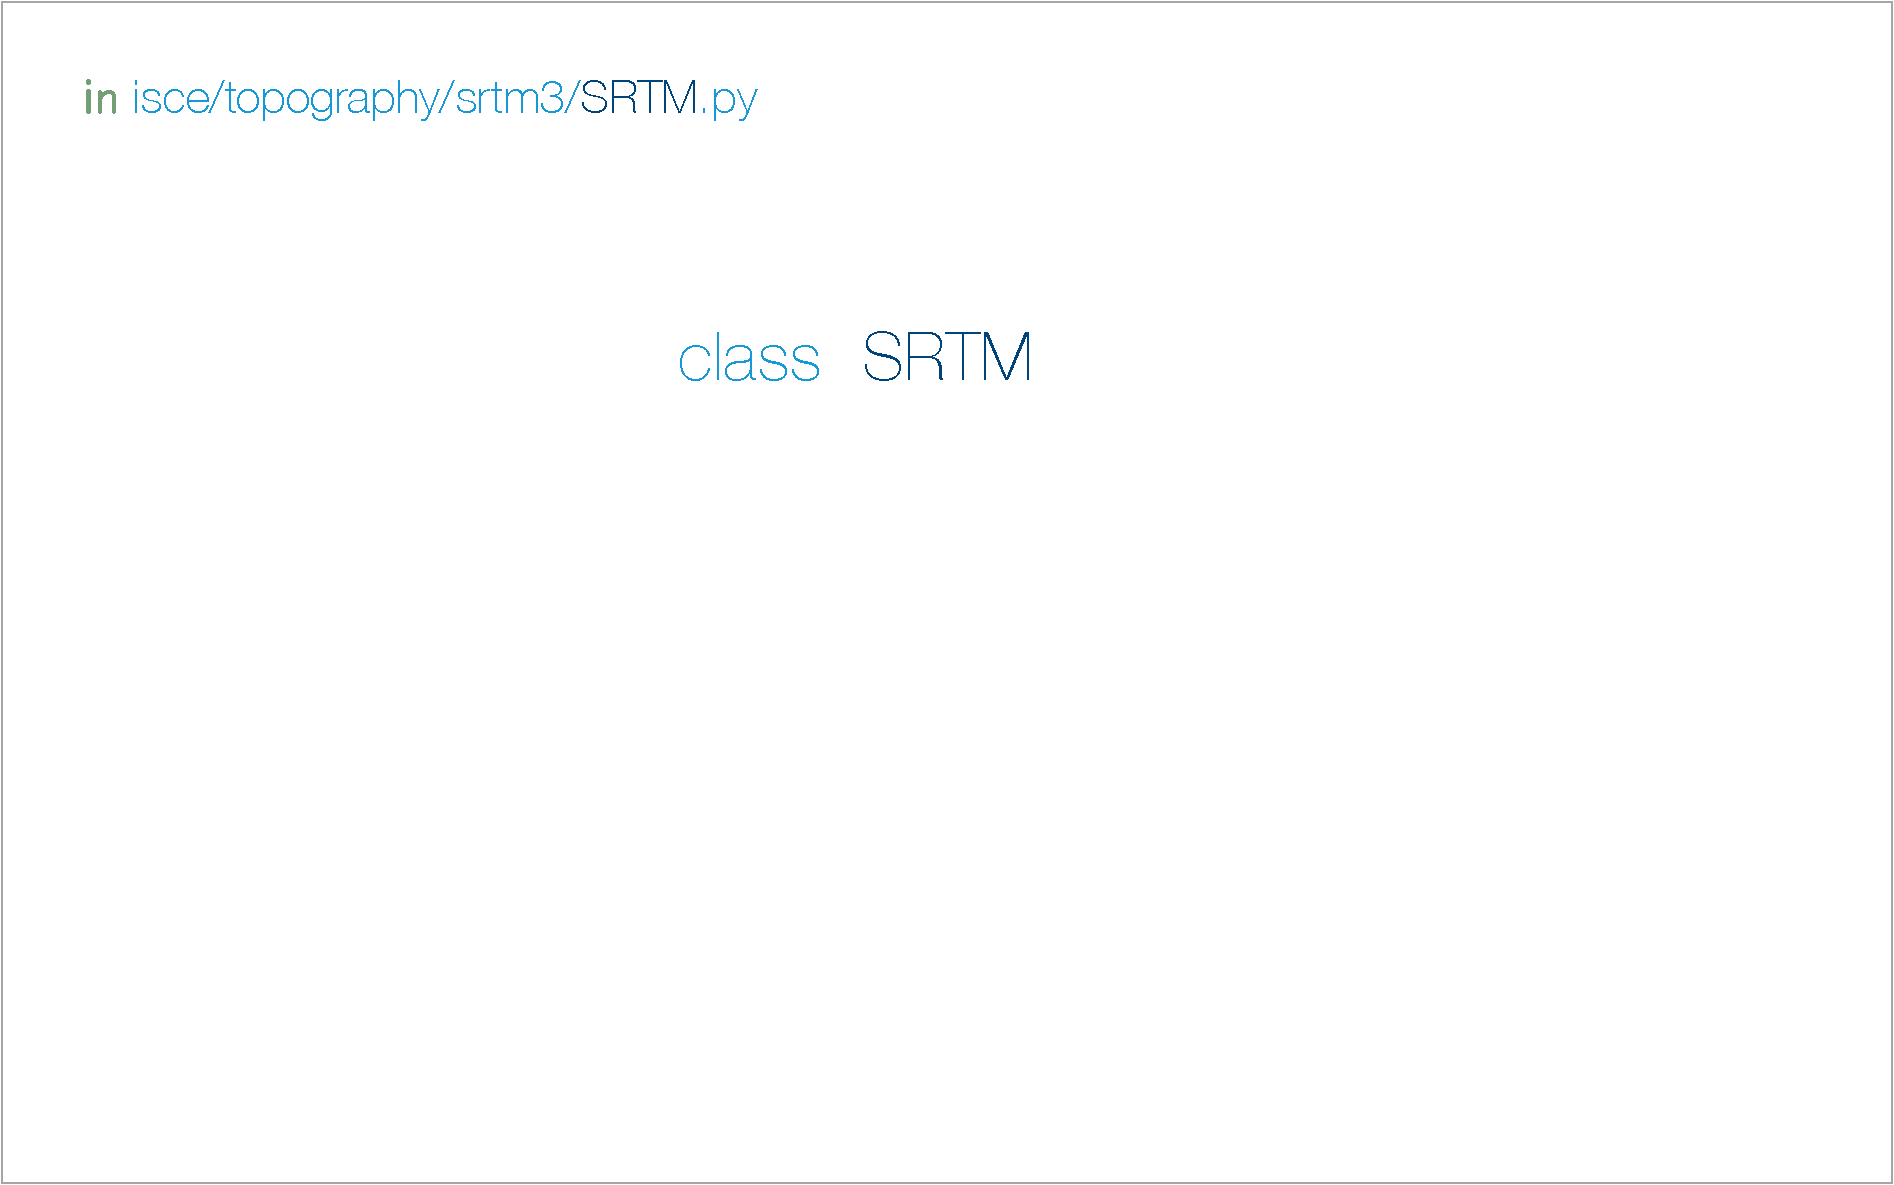
\includegraphics[width=1.0\textwidth]{component-package}}
    \only<2->{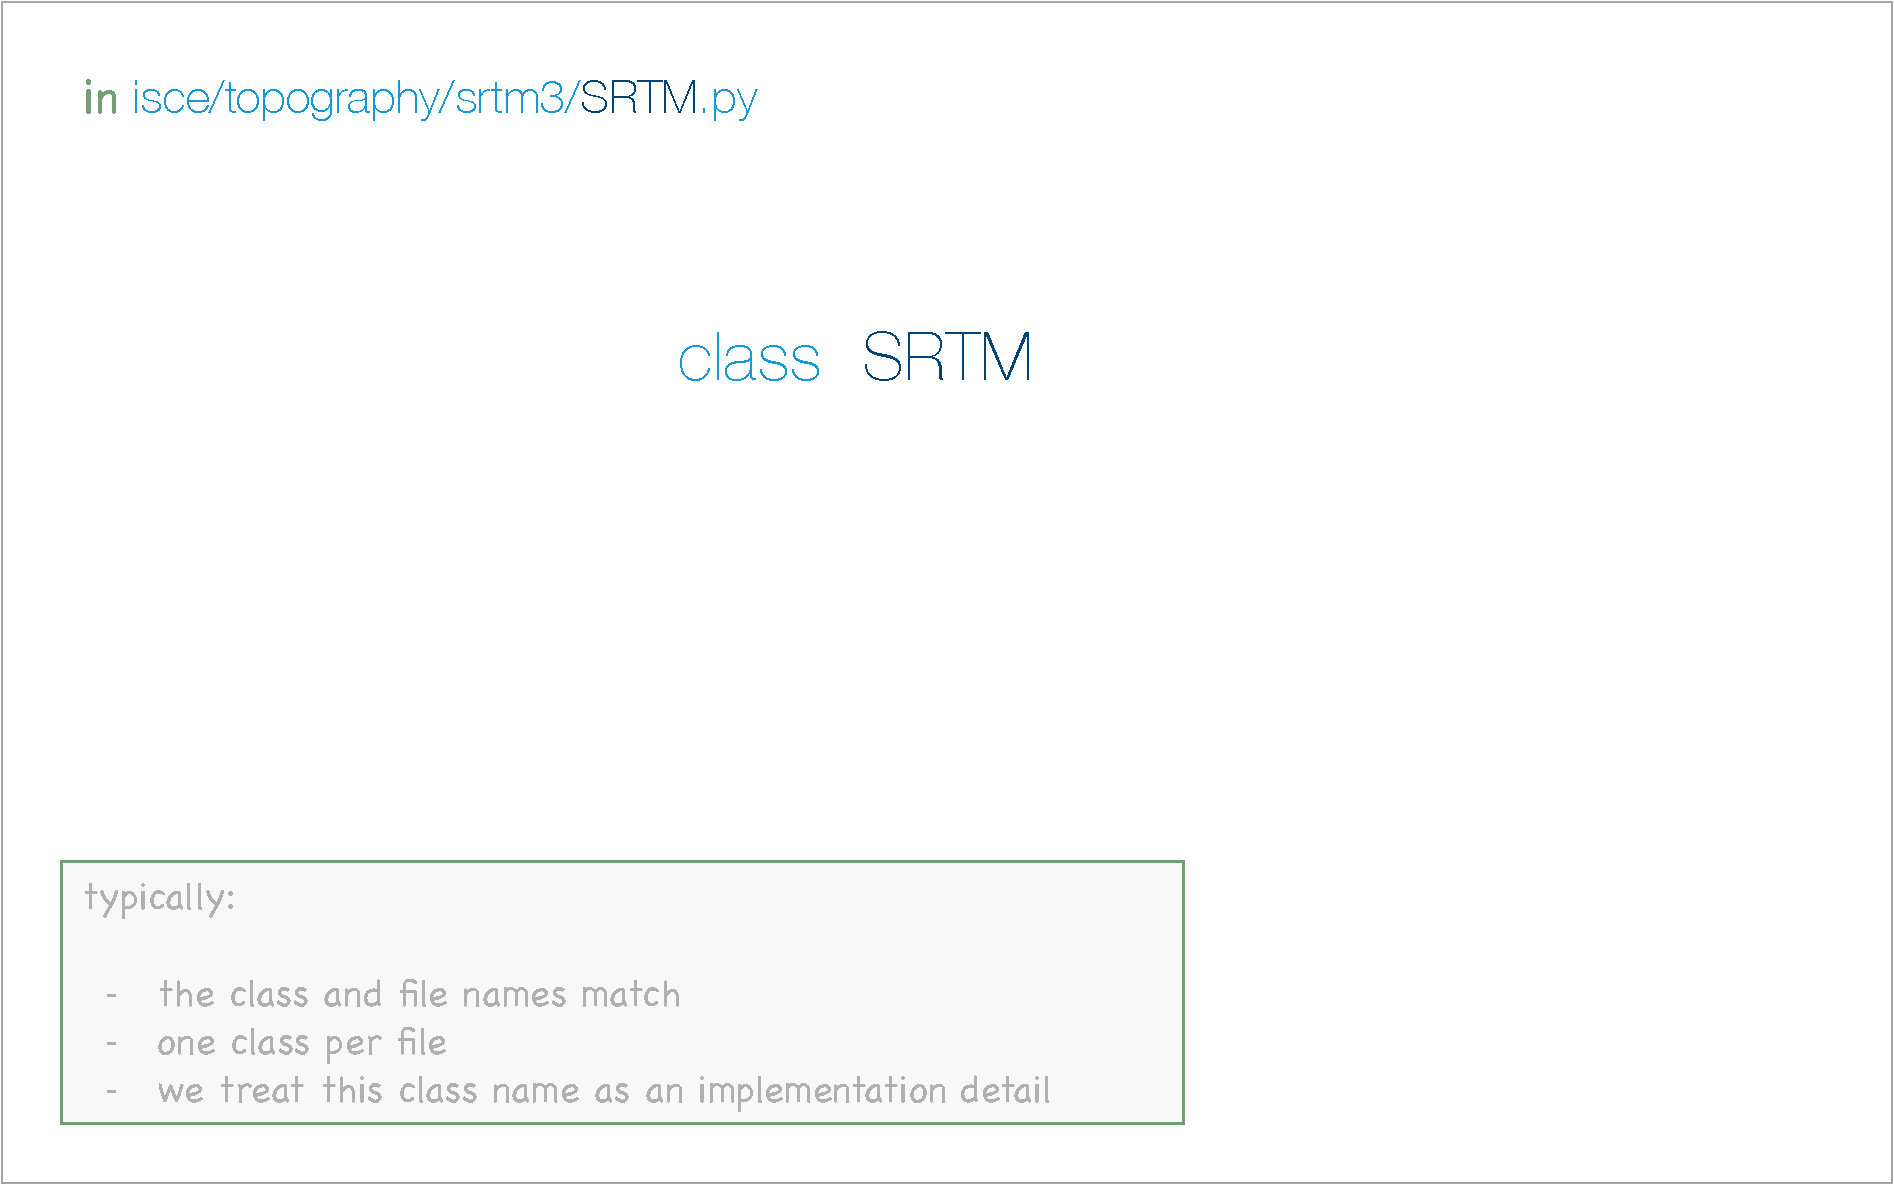
\includegraphics[width=1.0\textwidth]{component-package-explained}}
  \end{center}
%
\end{frame}

%-----------------------------------
\begin{frame}
%
  \frametitle{Turning classes into components}
%
  \begin{center}
    \only<1>{
\includegraphics[width=1.0\textwidth]{component-base}}
    \only<2>{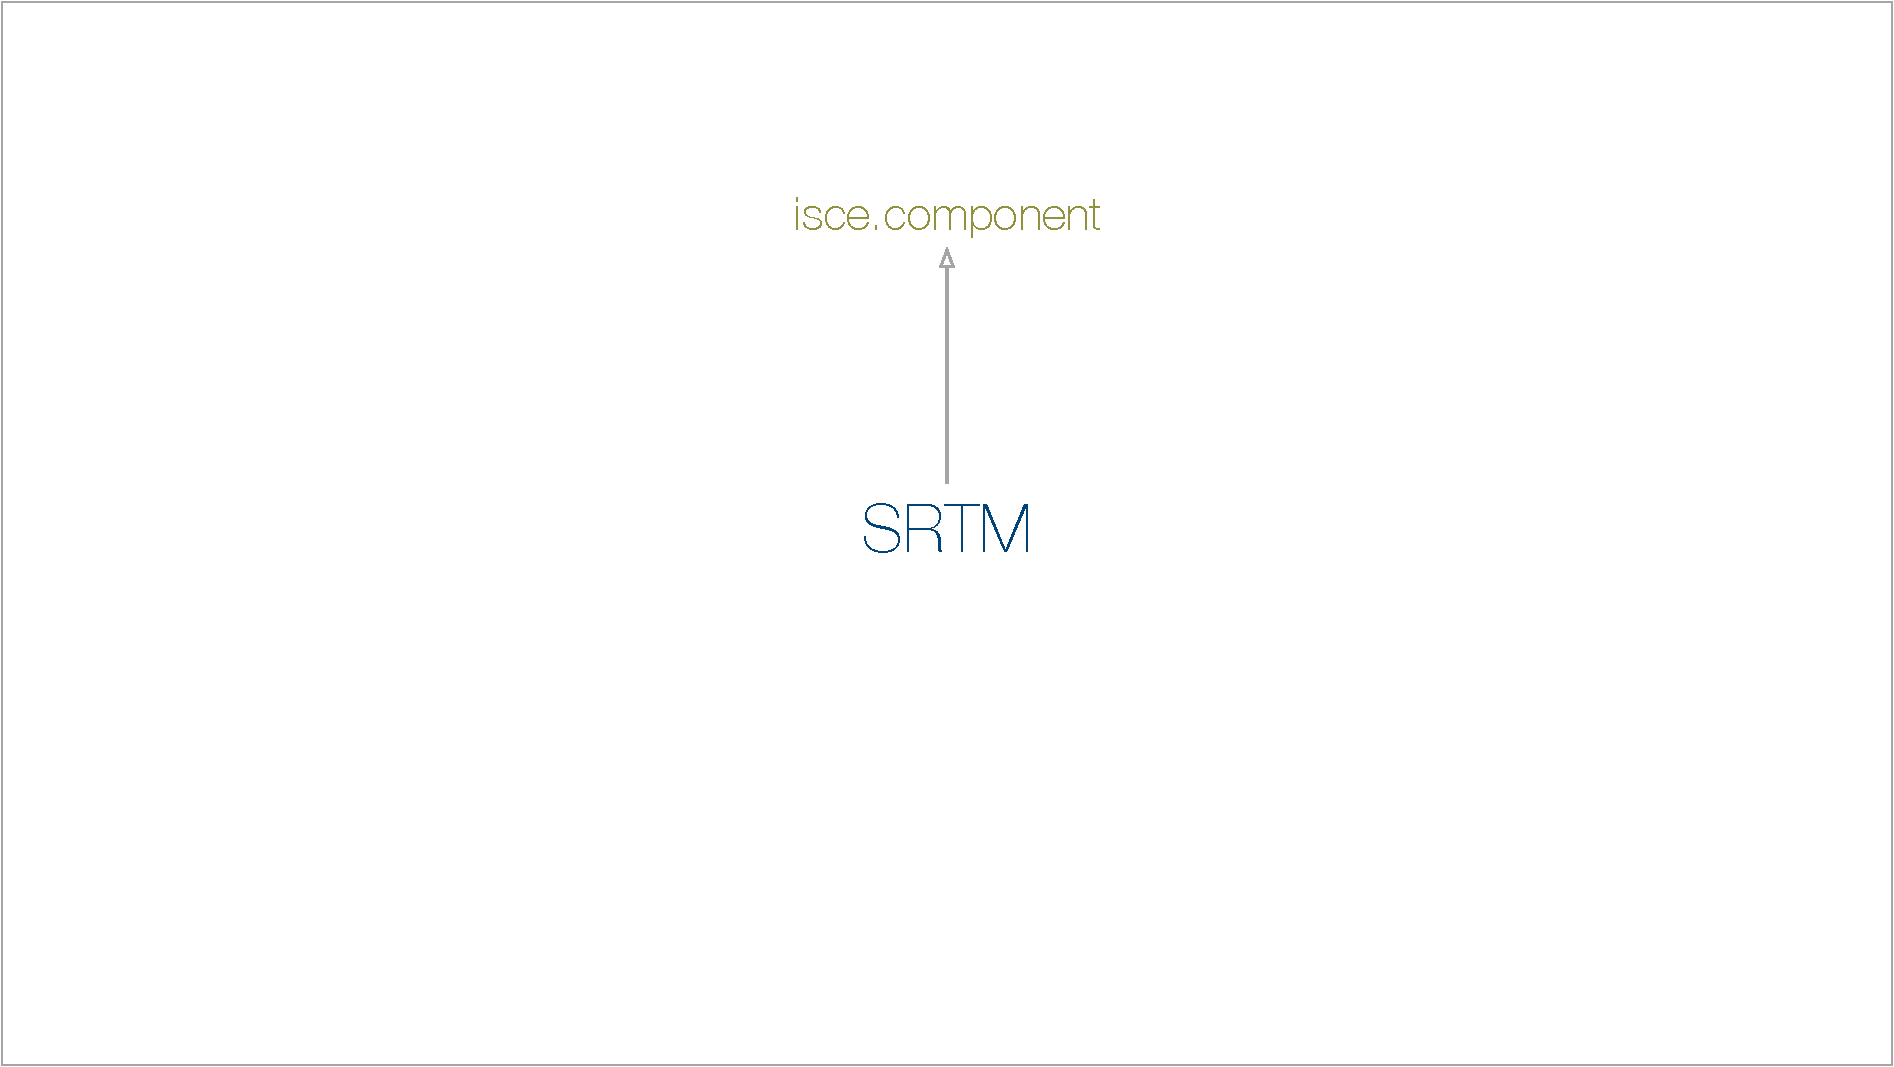
\includegraphics[width=1.0\textwidth]{component-inheritance}}
    \only<3>{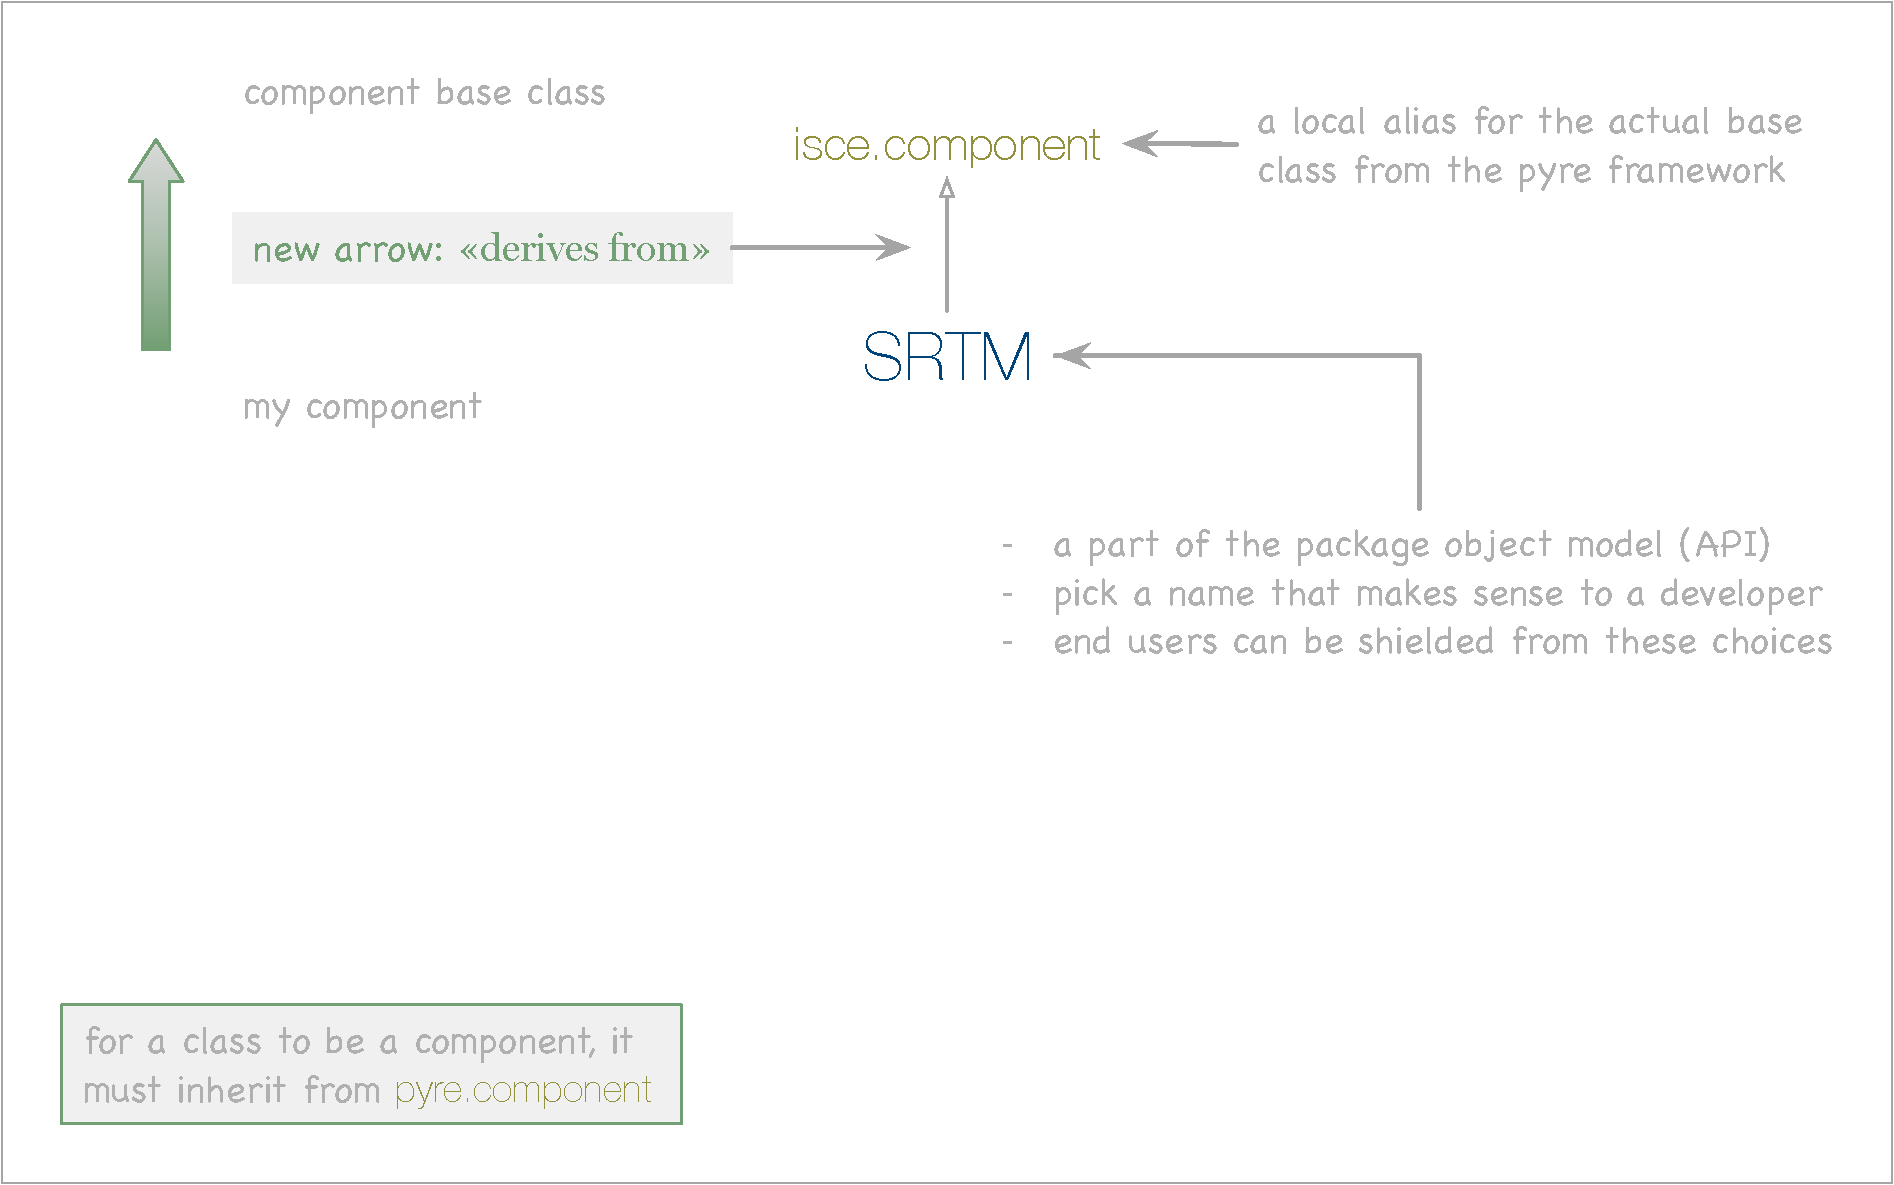
\includegraphics[width=1.0\textwidth]{component-inheritance-explained}}
  \end{center}
%
\end{frame}

%-----------------------------------
\begin{frame}[fragile]
%
  \frametitle{Component declaration}
%
  \vskip -3ex
  \begin{itemize}
%
  \item the instruction
    \begin{center}
      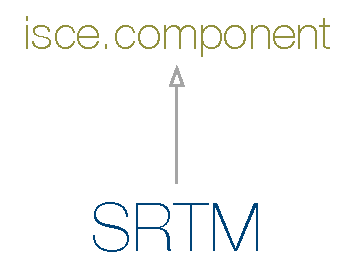
\includegraphics[height=10ex]{srtm-pedigree}
    \end{center}
%
  \item implies that instead of
%
    \begin{ipython}{}
class SRTM:
    """
    Access the SRTM data archive to download tiles and produce
    a digital elevation model for a specified region of interest
    """
    \end{ipython}
%
  \item we have to import the \isce\ package and derive from \class{isce.component}:
    \begin{ipython}{}
# support
import isce

# the srtm component
class SRTM(isce.component):
    """
    Access the SRTM data archive to download tiles and produce
    a digital elevation model for a specified region of interest
    """
    \end{ipython}
%
  \end{itemize}
%
\end{frame}

% --------------------------------------
% properties
\begin{frame}[fragile]
%
  \frametitle{Specifying the tile resolution}
%
  \begin{itemize}
%
  \item version 3 \srtm\ tiles come in two resolutions; enable the user to choose
%
    \begin{ipython}[firstnumber=4]{}
# the srtm component
class SRTM(isce.component):
    """
    Access the SRTM data archive to download tiles and produce
    a digital elevation model for a specified region of interest
    """

    # user configurable state
    resolution = 1 # arc seconds per pixel

    \end{ipython}
%
  \item how do we read the value of \trait{resolution} from a configuration file?
%
    \begin{ipfg}{}
      srtm:
          resolution = 1 ; arc seconds per pixel
    \end{ipfg}
%
    or, equivalently, from the command line of some driver script?
%
    \begin{ish}{}
      dem.py --srtm.resolution=1
    \end{ish}
%
  \item and resolve conflicts when different sources specify different values?
%
  \end{itemize}
%
\end{frame}

% --------------------------------------
% properties
\begin{frame}
%
  \frametitle{Components have properties}
%
  \begin{center}
    \only<1>{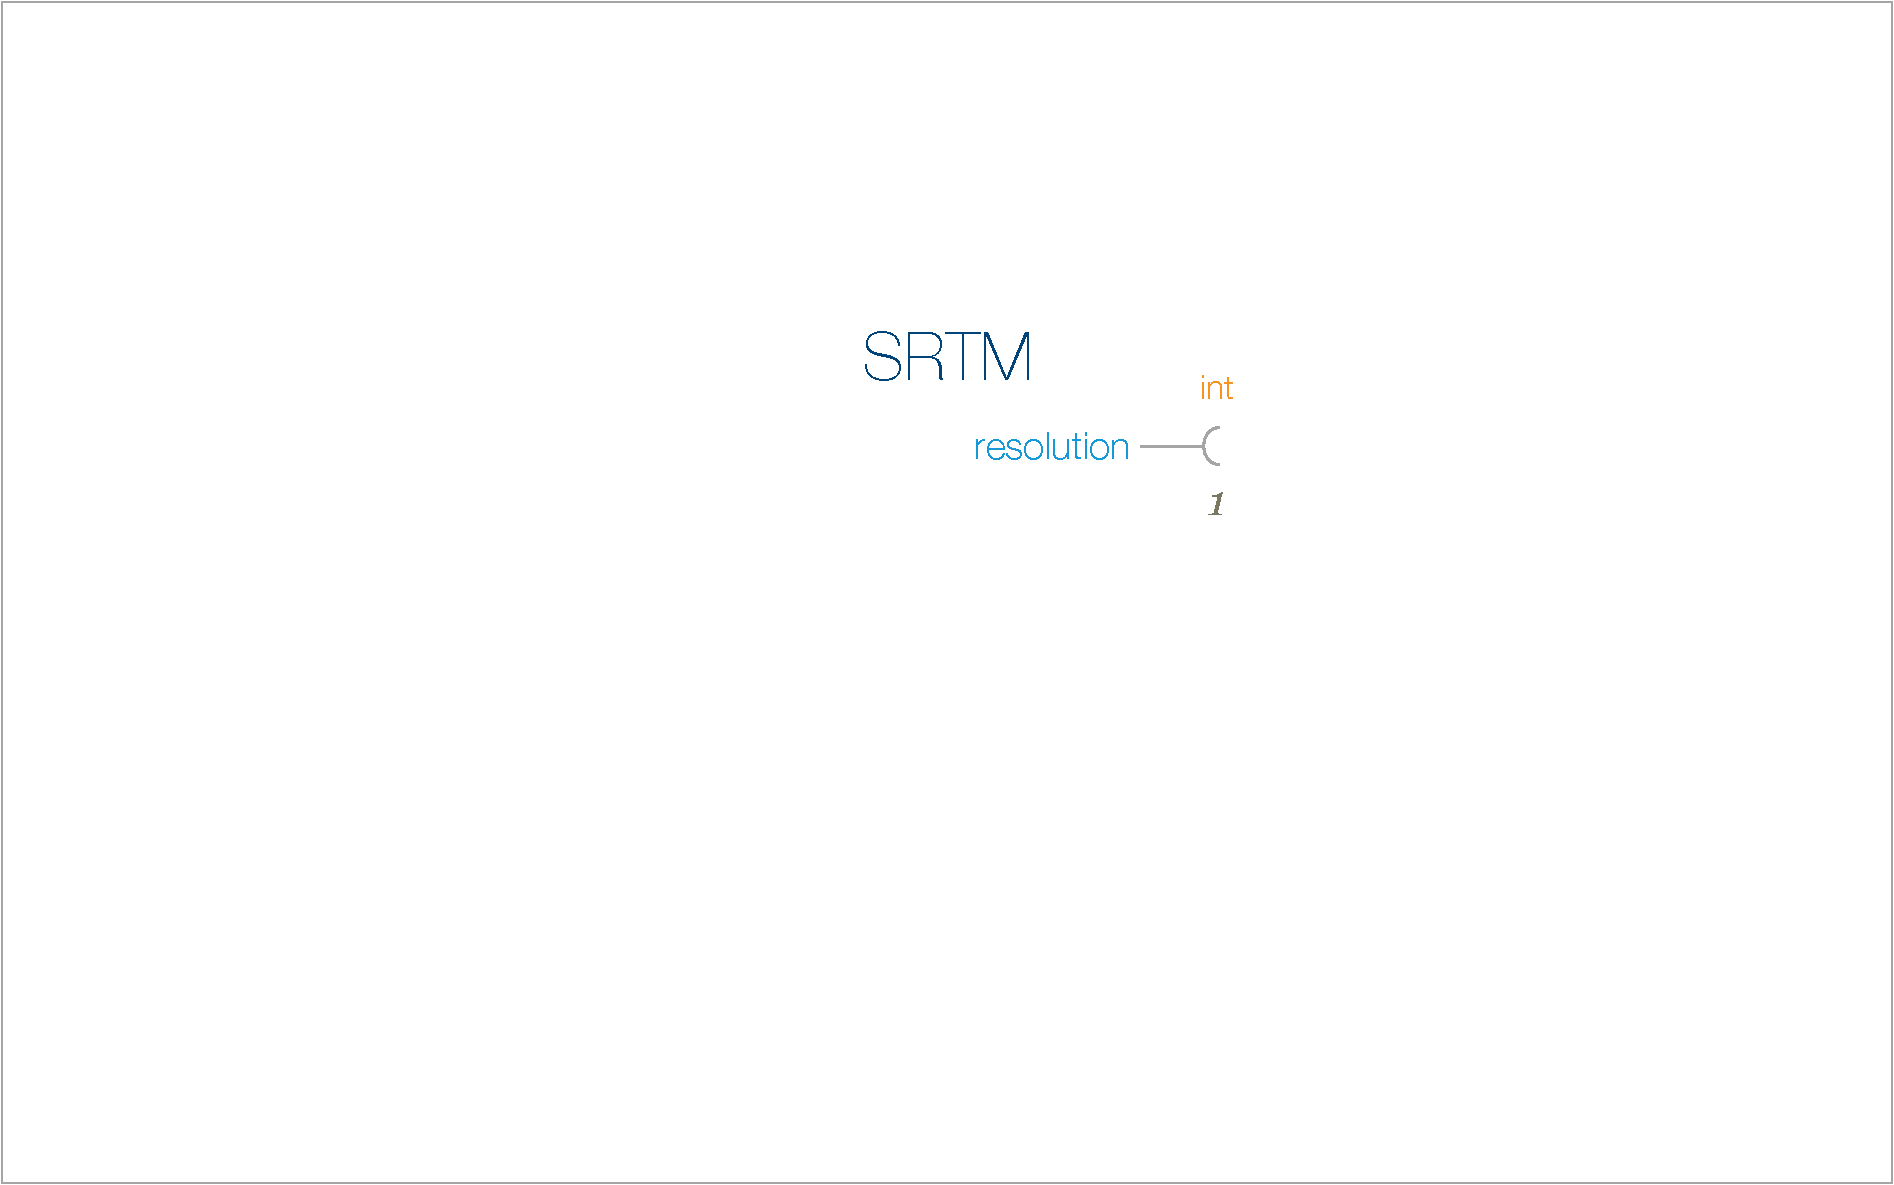
\includegraphics[width=1.0\textwidth]{component-properties}}
    \only<2->{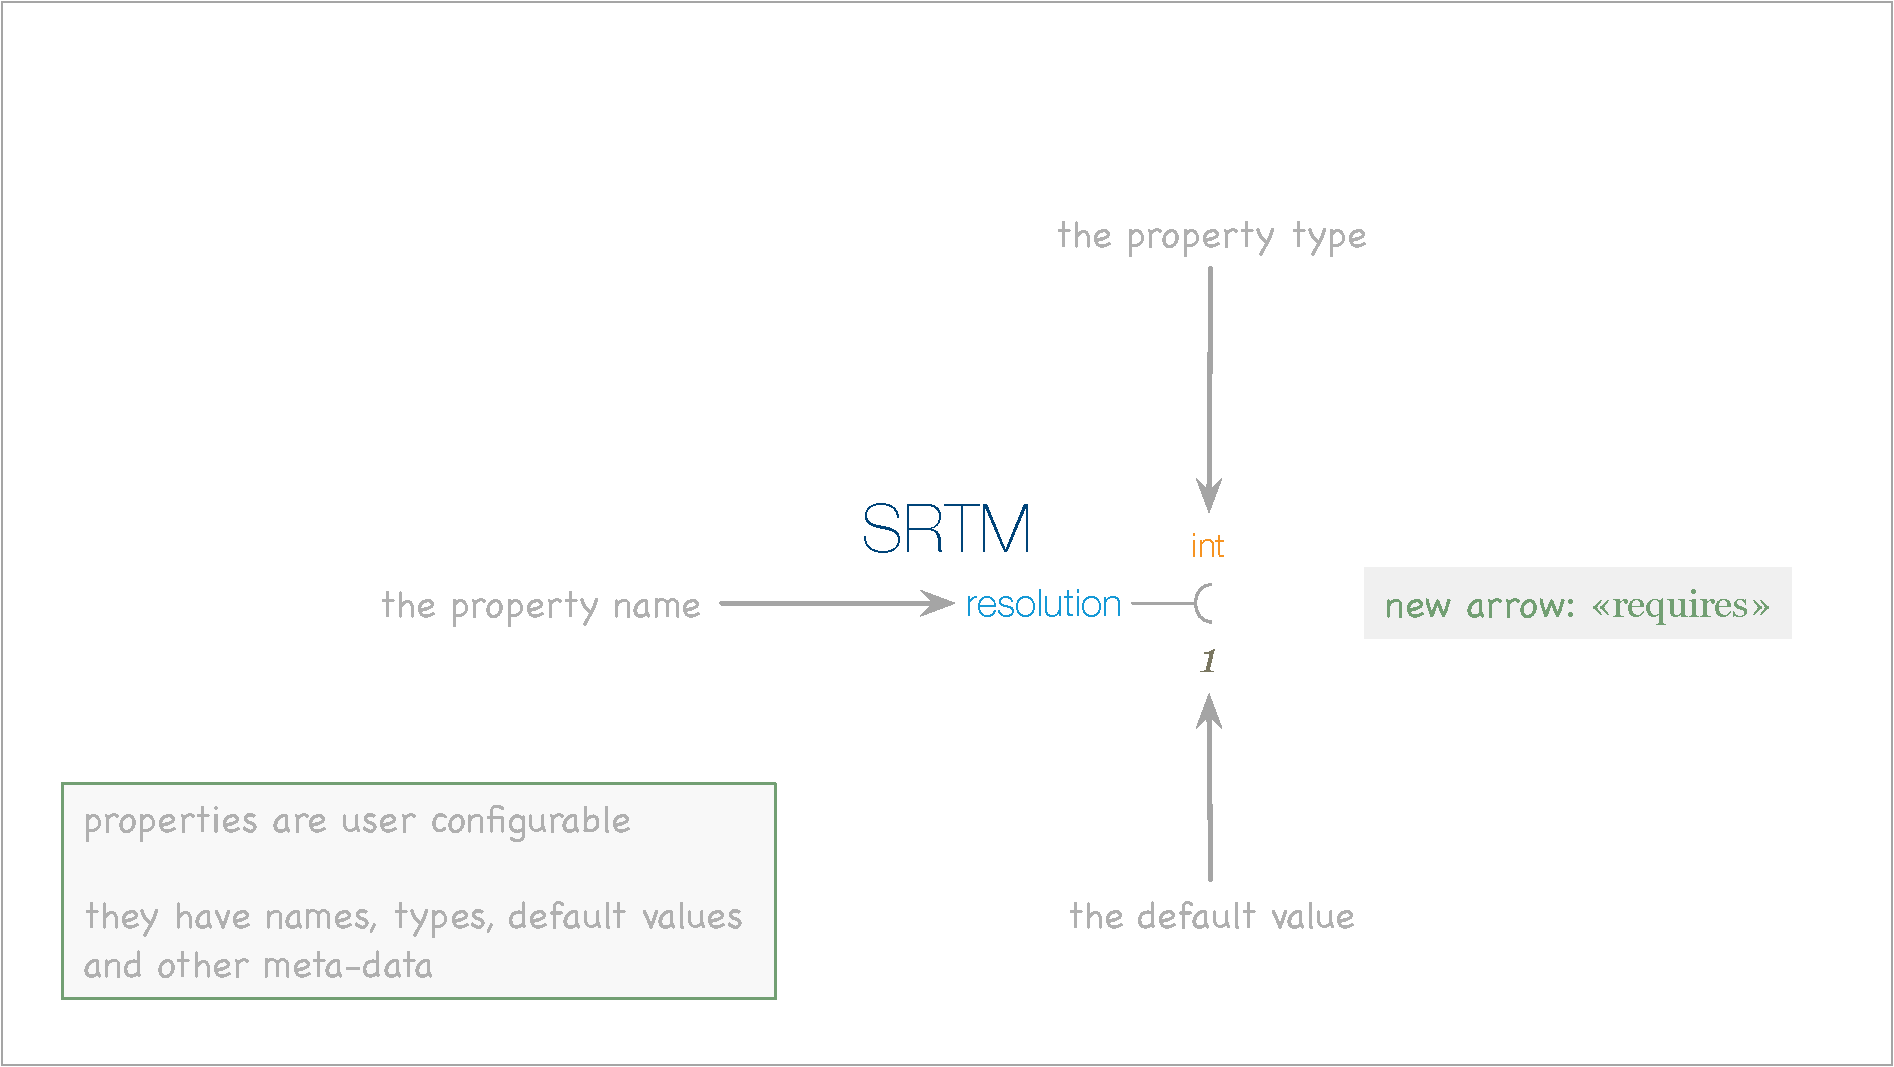
\includegraphics[width=1.0\textwidth]{component-properties-explained}}
  \end{center}
%
\end{frame}

% --------------------------------------
\begin{frame}[fragile]
%
  \frametitle{Adding properties to a component}
%
  \vskip -4ex
  \begin{itemize}
%
  \item the instruction
%
    \begin{center}
      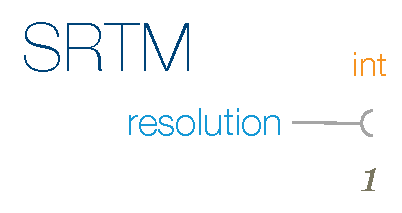
\includegraphics[height=10ex]{srtm-resolution}
    \end{center}
%
  \item implies the following modification to the \class{SRTM} declaration:
%
    \begin{ipython}[firstnumber=4]{}
# the srtm component
class SRTM(isce.component):
    """
    Access the SRTM data archive to download tiles and produce
    a digital elevation model for a specified region of interest
    """

    # user configurable state
    resolution = isce.properties.int(default=1)
    resolution.doc = 'the tile resolution in arc seconds per pixel'

    \end{ipython}
%
  \item why bother specifying the type of component properties?
    \begin{itemize}
    \item command line, configuration files, dialog boxes, web pages: they all gather
      information from the user as strings
    \item we need \emph{meta-data} so we can convert from strings to the intended object
    \end{itemize}
%
  \end{itemize}
%
\end{frame}

% --------------------------------------
\begin{frame}
%
  \frametitle{Properties}
%
  \vskip -2ex
  \begin{itemize}
%
  \item properties make sense for both classes and instances
    \begin{itemize}
    \item the class holds the default value that gets used in case the component instance does
      not have explicit configuration
    \item each instance gets its own private value when it gets configured
    \item the behavior is identical to regular python attributes
    \end{itemize}
%
  \item there is support for
    \begin{itemize}
    \item simple types: \function{bool}, \function{int}, \function{float}, \function{str}
    \item containers: \function{tuple}, \function{list}, \function{set}, \function{array}
    \item higher level: \function{date}, \function{time}, \function{istream},
      \function{ostream}, \function{inet}
    \item units: \function{dimensional}
    \item easy enough to implement your own; the requirements are very simple
    \end{itemize}
%
  \item metadata:
    \begin{itemize}
    \item \identifier{doc} and \identifier{tip}: simple and short documentation strings
    \item \identifier{default}: the default value, in case the user doesn't supply one
    \item \identifier{converters}: a chain of preprocessors of the string representation
    \item \identifier{normalizers}: a chain of post-processors of the converted value
    \item \identifier{validators}: a tuple of predicates that get called to ensure the property
      value satisfies the specified constraints
    \item you can add your own; the framework passes them through to your component
    \end{itemize}
%
  \end{itemize}
%
\end{frame}

% --------------------------------------
% units
\begin{frame}[fragile]
%
  \frametitle{Units}
%
  \vskip -2ex
  \begin{itemize}
%
  \item \function{dimensional} properties have units
%
  \item the low level support is in \package{pyre.units}
    \begin{itemize}
    \item full support for all SI base and derived units
    \item all common abbreviations and names from alternative systems of units
    \item correct arithmetic; proper handling of functions from \package{math}
    \end{itemize}
%
  \item consider
    \begin{ipython}{}
from math import cos
from pyre.units.SI import meter, second, radian

A = 2.5 * meter
t = 1.5 * second
ω = 4.2 * radian/second

x = A * cos(ω * t)
     \end{ipython}
%
   \item if the units in the argument to \function{cos} do not cancel, leaving a pure
     \keyword{float} behind, an exception is raised; \identifier{x} has dimensions of meters
%
  \end{itemize}
%
\end{frame}

%-----------------------------------

\begin{frame}[fragile]
%
  \frametitle{A slightly more complicated example}
%
  \vskip -4ex
  \begin{itemize}
%
  \item let's add the \trait{region} requirement
%
    \begin{center}
      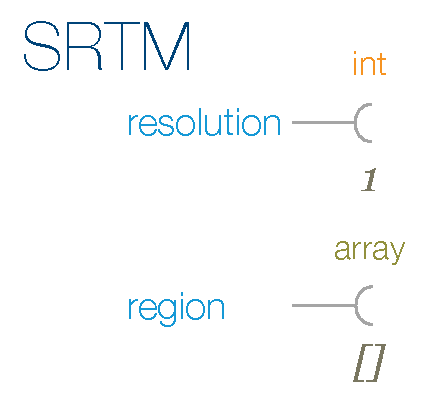
\includegraphics[height=15ex]{srtm-region}
    \end{center}
%
  \item the \class{SRTM} declaration becomes:
%
    \begin{ipython}[firstnumber=4]{}
# the srtm component
class SRTM(isce.component):
    """
    Access the SRTM data archive to download tiles and produce
    a digital elevation model for a specified region of interest
    """

    # user configurable state
    resolution = isce.properties.int(default=1)
    resolution.doc = 'the tile resolution in arc seconds per pixel'

    region = isce.properties.array()
    region.doc = 'a cloud of (lat,lon) pairs'

    \end{ipython}
%
  \end{itemize}
%
\end{frame}

%-----------------------------------

\begin{frame}
%
  \frametitle{More notation}
%
  \begin{itemize}
%
  \item Sometimes we need to communicate the values to which properties are bound:

      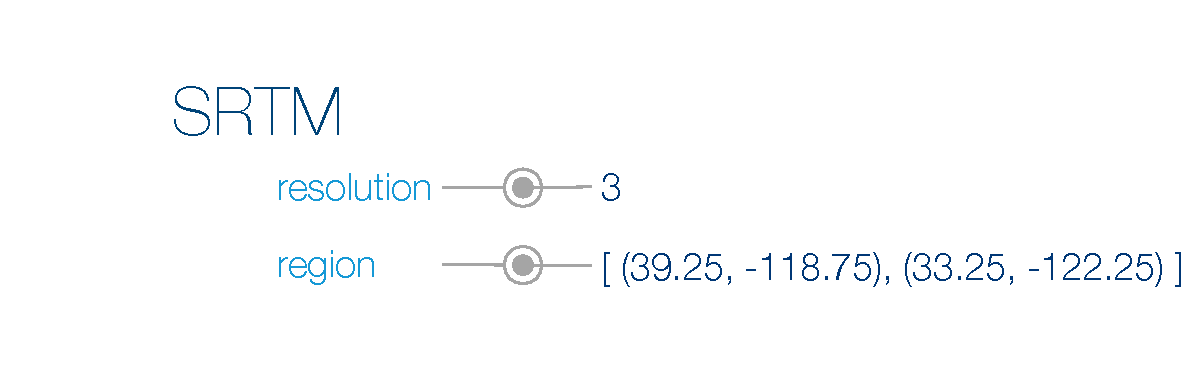
\includegraphics[height=20ex]{srtm-properties-bound}

  \item a more compact alternative to the property declarations

      
\includegraphics[height=10ex]{srtm-properties-compact}

    for when we don't care to show the binding slots
%
  \end{itemize}
%
\end{frame}

%-----------------------------------
\begin{frame}
%
  \frametitle{SRTM -- family}
%
  \begin{center}
    \only<1>{
\includegraphics[width=1.0\textwidth]{component-family}}
    \only<2>{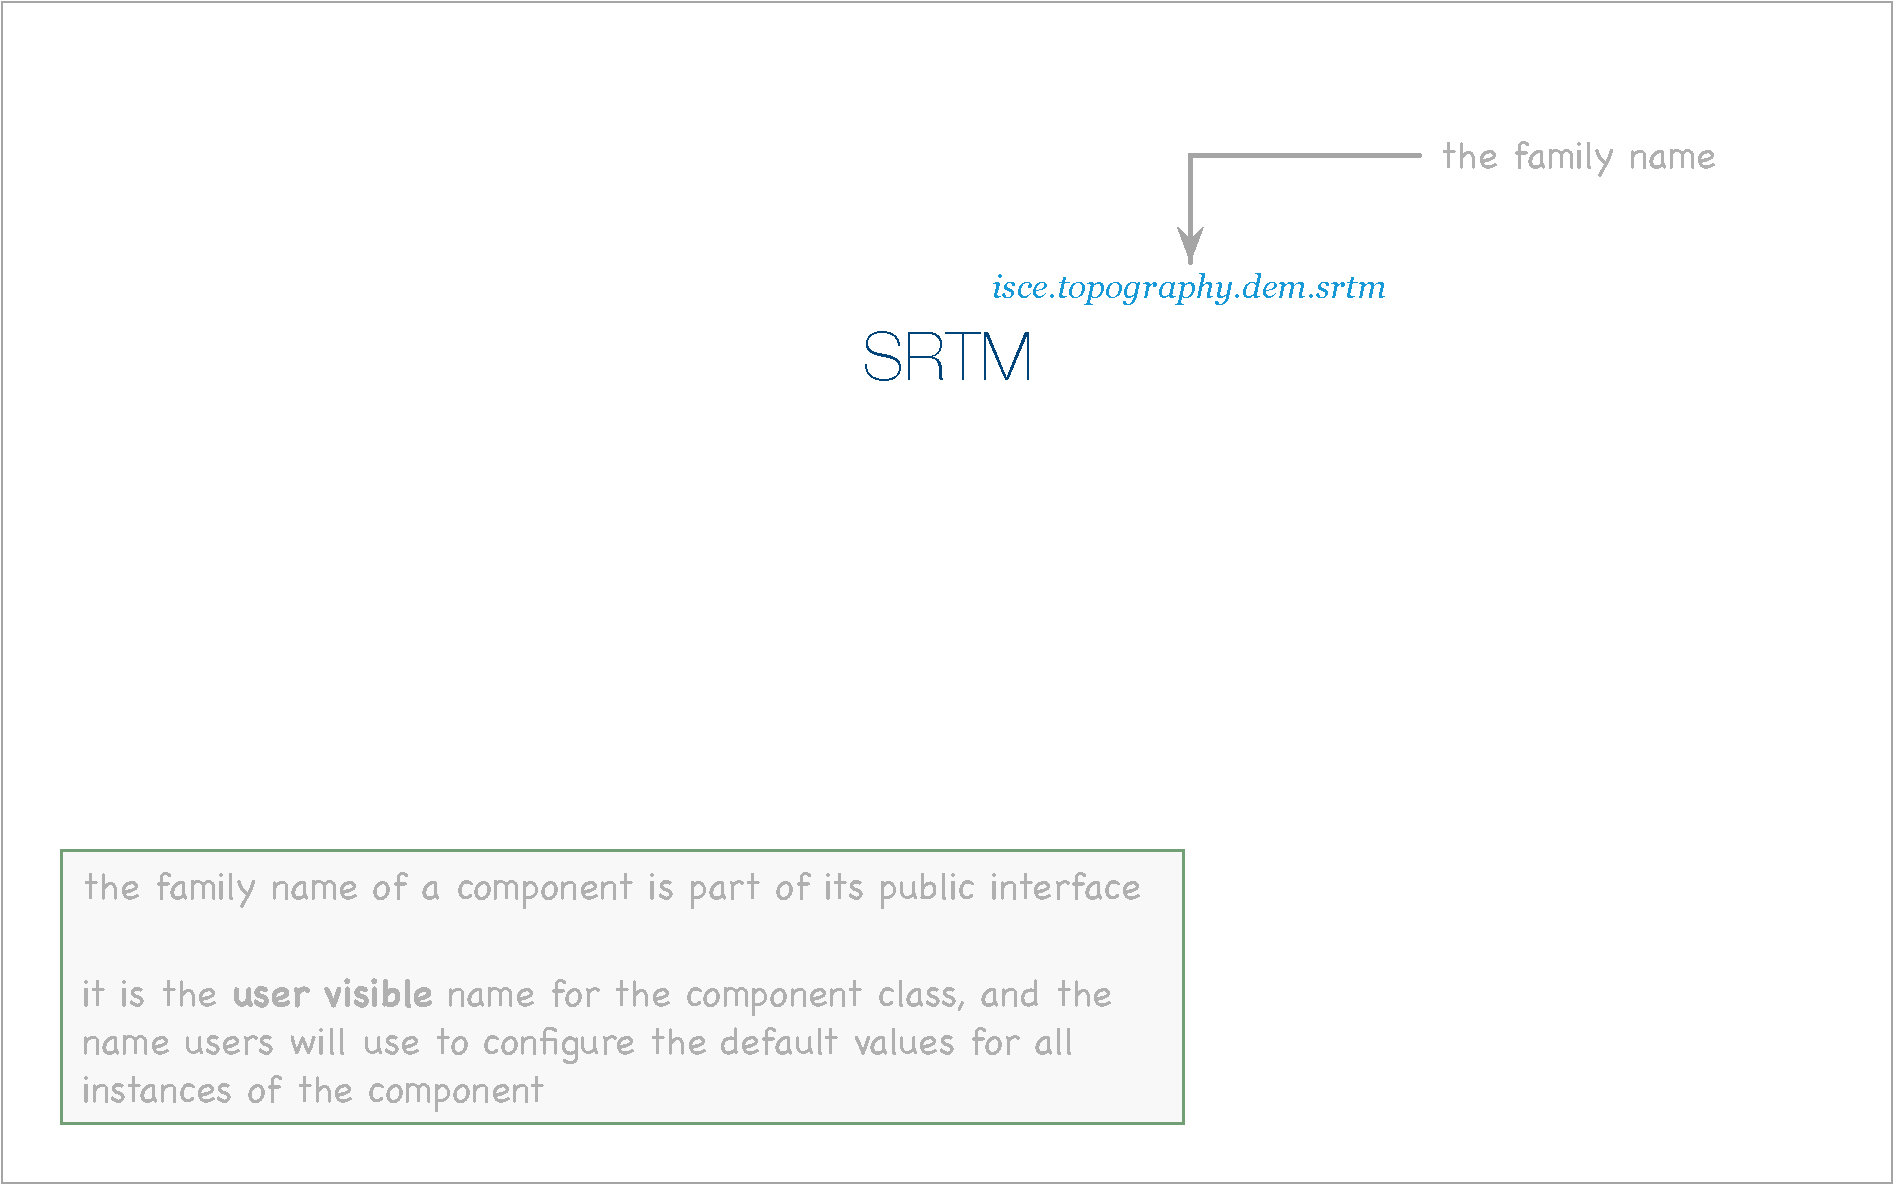
\includegraphics[width=1.0\textwidth]{component-family-explained}}
  \end{center}
%
\end{frame}

%-----------------------------------
\begin{frame}
%
  \frametitle{SRTM - protocol}
%
  \begin{center}
    \only<1>{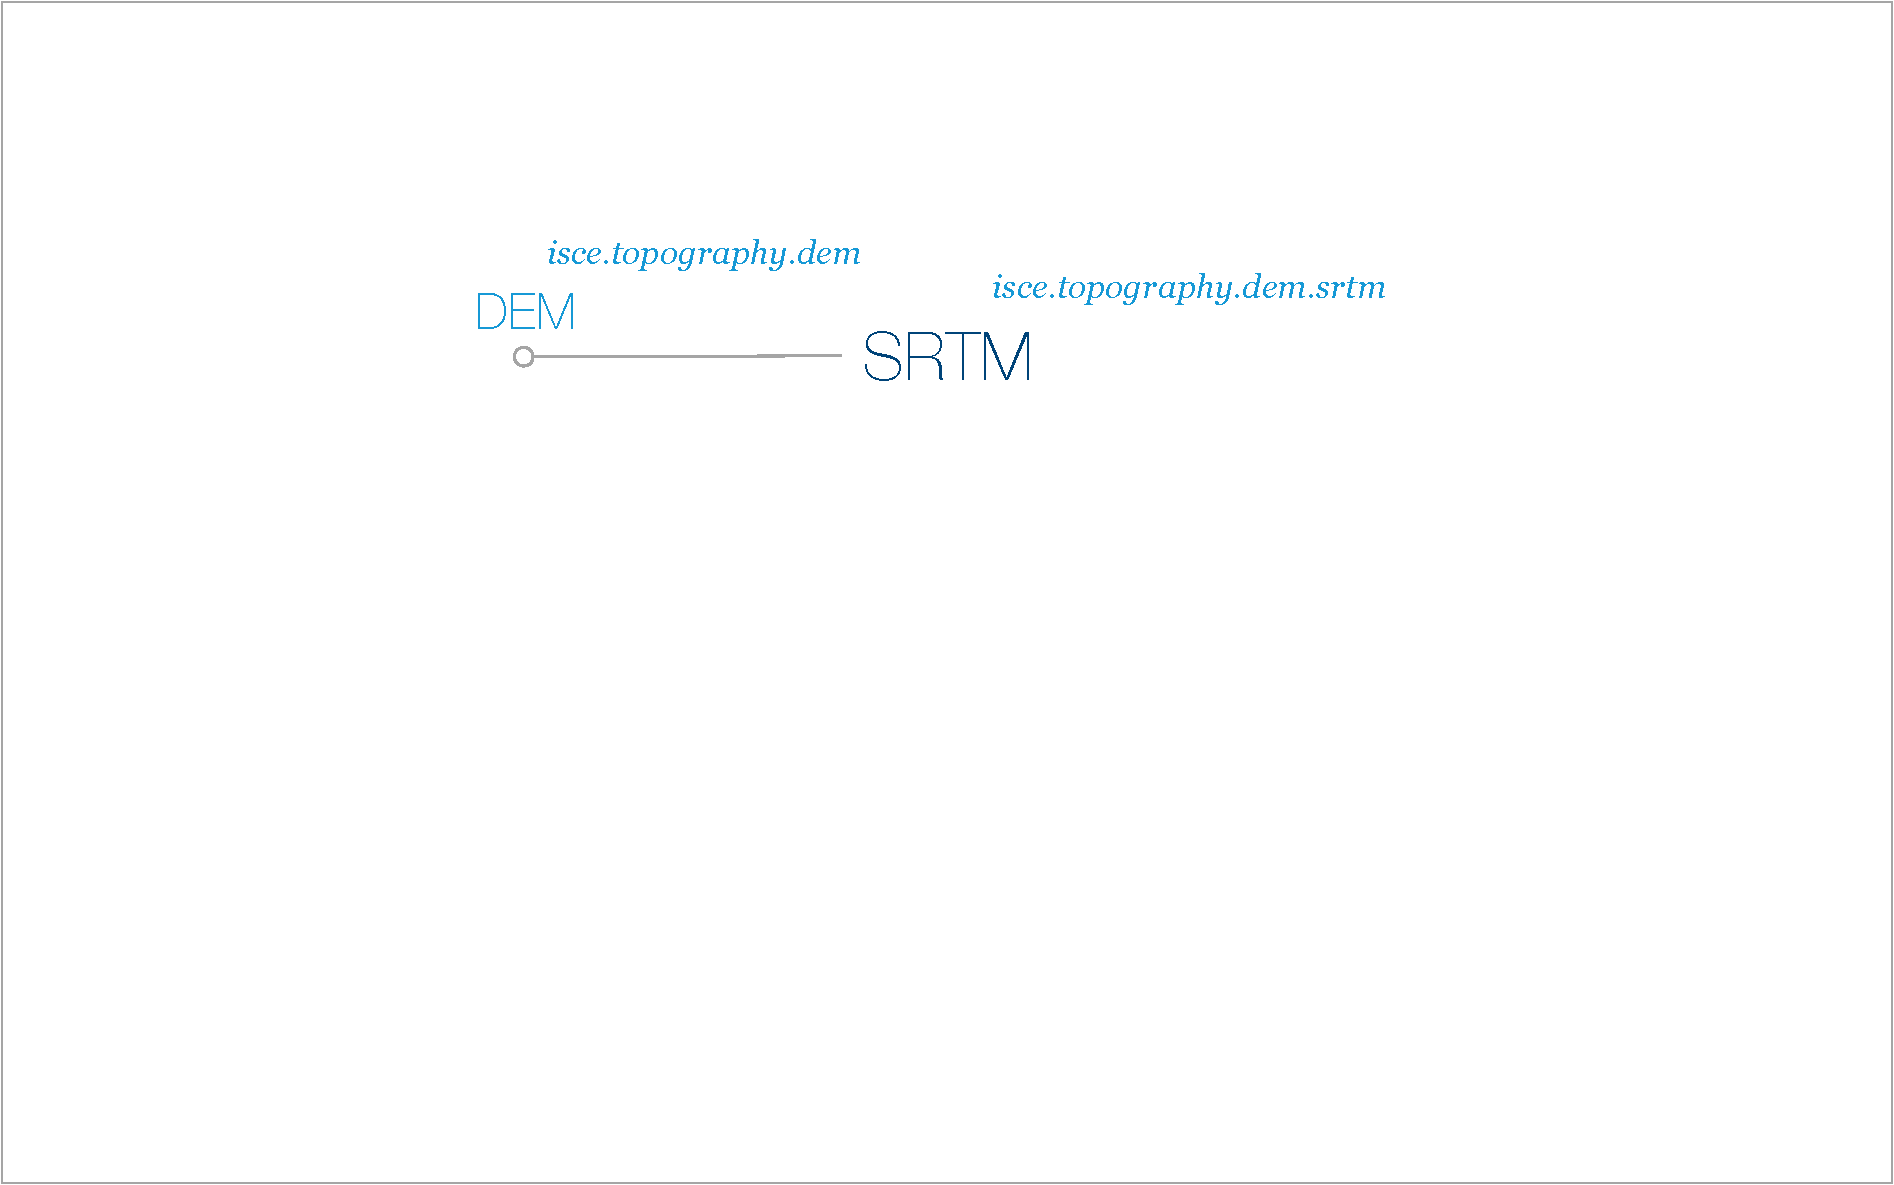
\includegraphics[width=1.0\textwidth]{component-implements}}
    \only<2>{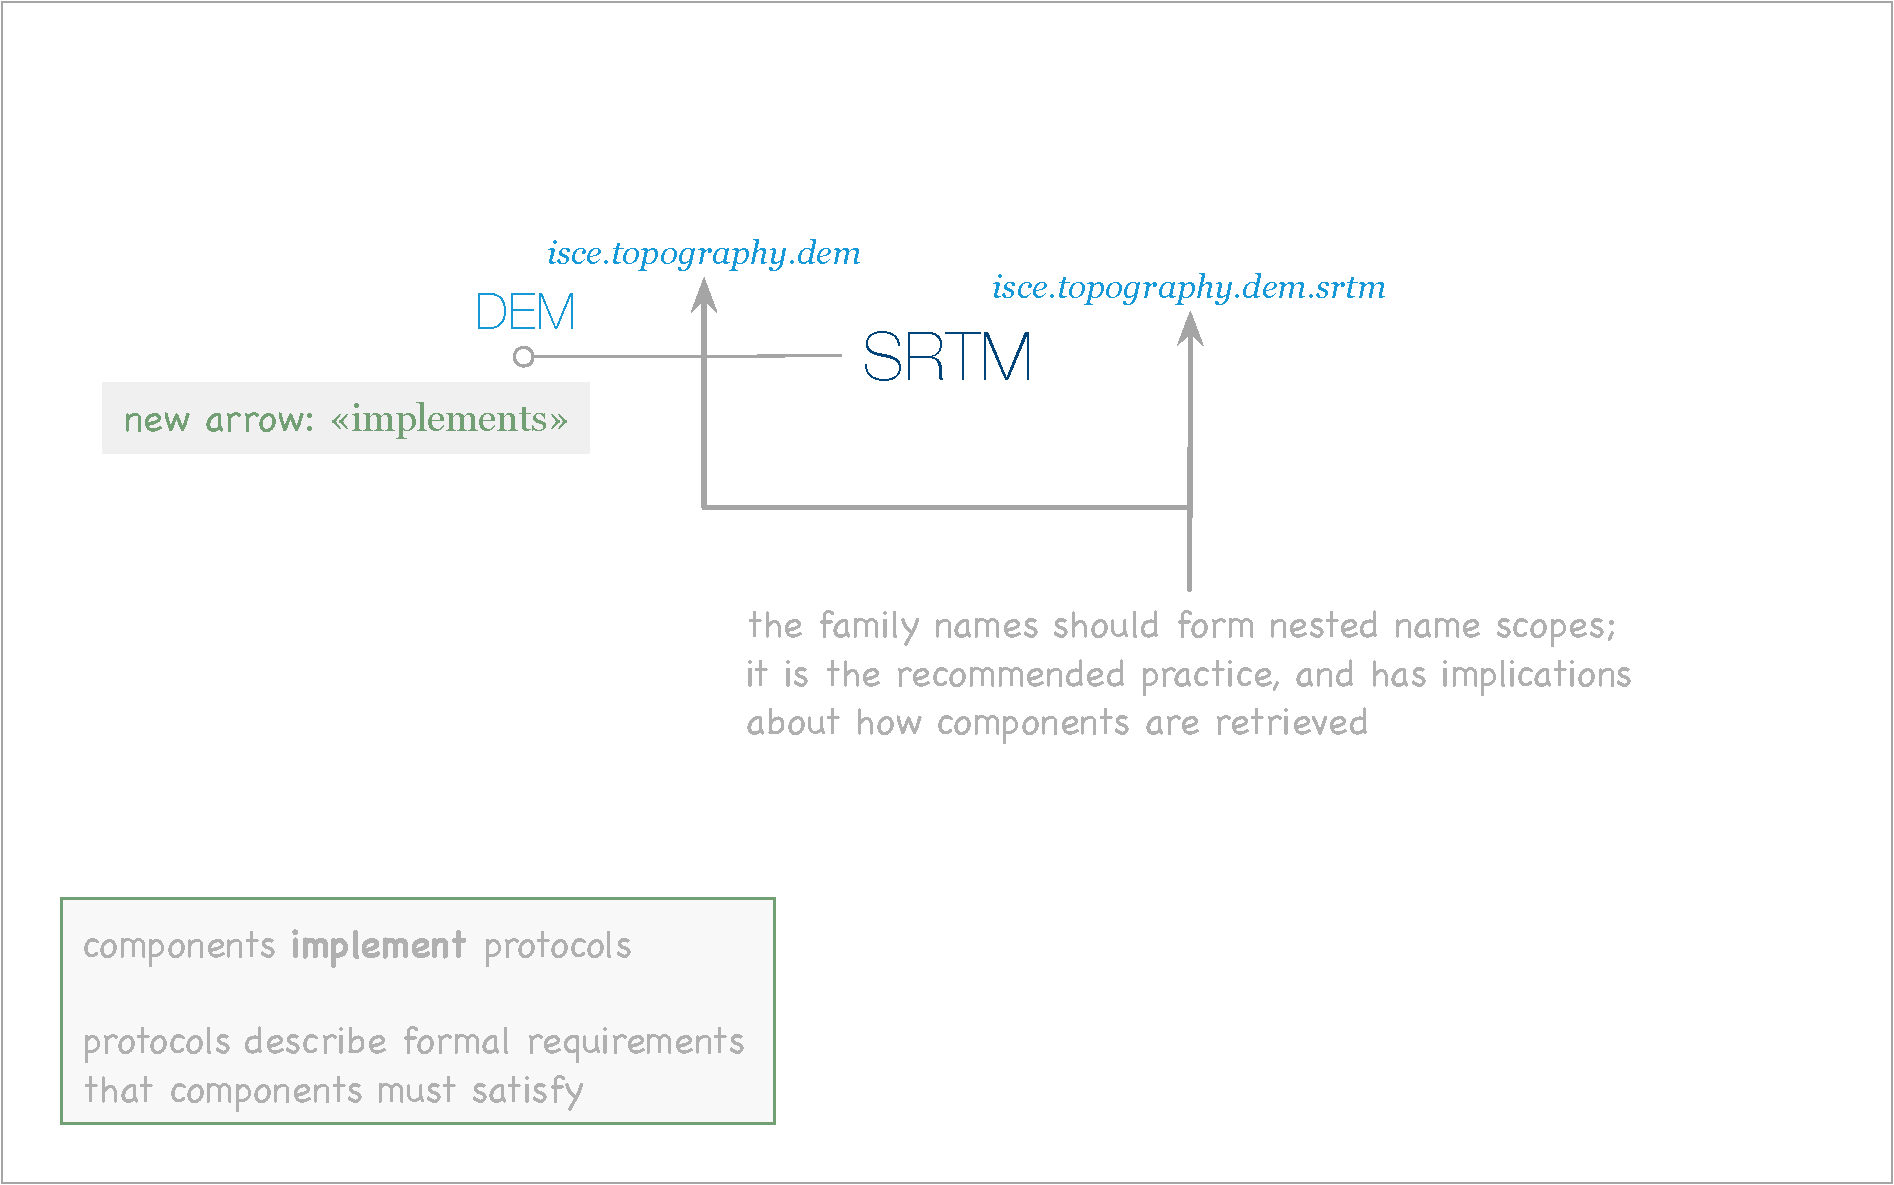
\includegraphics[width=1.0\textwidth]{component-implements-explained}}
  \end{center}
%
\end{frame}

% --------------------------------------
% recap
\begin{frame}
%
  \frametitle{Recap: what we know so far}
%
  \begin{itemize}
%
  \item \pyre\ components are evolved python objects
    \begin{itemize}
    \item the classes have family names, the instances have names
    \item these names are unique strings in hierarchical namespaces delimited by periods
    \item collections of components form packages \emph{implicitly}, based on the topmost level
      in their namespace
    \end{itemize}
%
  \item components have properties that are under the control of the \emph{user}
    \begin{itemize}
    \item they look and behave like regular attributes
    \item they are \emph{typed} to enable conversions from strings
    \item they have default values and other metadata
    \end{itemize}
%
  \item configuration is partly about assigning values to component properties
    \begin{itemize}
    \item a requirement for supporting user interfaces
    \item intuitive syntax for the command line
    \item simple configuration files in a variety of formats: \identifier{XML}, Microsoft
      Windows \identifier{.ini}, native \identifier{.pfg}
    \end{itemize}
%
  \item configuration is automatically handled by the framework and requires no explicit
    involvement on the part of the component author
%
  \end{itemize}
%
\end{frame}

% --------------------------------------
\begin{frame}
%
  \frametitle{Components and protocols}
%
  \begin{itemize}
%
  \item a design pattern\supercite{patterns} that enables the assembly of applications out of
    interchangeable parts, under the control of the end user
      \begin{itemize}
      \item \emph{protocols} are abstract specifications of application requirements
      \item \emph{components} are concrete implementations that satisfy requirements
      \end{itemize}
%
    \item protocols make it possible to write applications without any \emph{a priori} knowledge
      of implementation specifics
%
    \item inversion of control\supercite{johnson-88}:
      \begin{itemize}
      \item the binding of actual implementations to the application requirements happens at
        runtime, under the control of the end user
      \end{itemize}
%
    \item in \pyre, the user
      \begin{itemize}
      \item controls the application state through configuration files, the user interface, the
        command line
      \item specifies components using simple URIs
      \end{itemize}
%
    \item the goal is to isolate contributors from each other as much as possible, and provide
      a coherent and usable strategy for composing non-trivial applications
%
  \end{itemize}
%
\end{frame}

%%% Local Variables:
%%% mode: latex
%%% TeX-master: "../pyre"
%%% End:

% end of file
